\documentclass[10pt]{beamer}

\usepackage[T2A]{fontenc}
\usepackage[utf8]{inputenc}
\usepackage[russian,english]{babel}

\usefonttheme[onlymath]{serif}

\usetheme[progressbar=frametitle]{metropolis}
\usepackage{appendixnumberbeamer}

\usepackage{booktabs}
\usepackage[scale=2]{ccicons}

\usepackage{pgfplots}
\usepgfplotslibrary{dateplot}

\usepackage{xspace}
\newcommand{\themename}{\textbf{\textsc{metropolis}}\xspace}
\newcommand{\TODO}[1]{\textbf{\textcolor{red}{TODO: #1}}}

\date{}
\author{Екатерина Тузова}


\title{Лекция 2}
\subtitle{Метрические классификаторы}

\begin{document}

\maketitle

\section{Разбор летучки}

\section{Мотивирующий пример}

{\foot{\href{https://www.kaggle.com/abcsds/pokemon}{Pokemon with stats (https://www.kaggle.com/abcsds/pokemon)}}
\begin{frame}{Мотивирующий пример}
	\begin{figure}
	    \centering
	    \subfloat{{
\includegraphics[width=2cm]{images/Bulbasaur} }}
	    \qquad
	    \subfloat{{
\includegraphics[width=2cm]{images/Mewtwo} }}
    	    \qquad
    	    \subfloat{{
\includegraphics[width=2cm]{images/Volcanion} }}
    	    \qquad
    	    \subfloat{{
\includegraphics[width=2cm]{images/Ekans} }}
    	    \qquad
    	    \subfloat{{
\includegraphics[width=2cm]{images/Nidorina} }}
	    \qquad 
    	    \subfloat{{
\includegraphics[width=2cm]{images/Rattata} }}
	    \qquad
    	    \subfloat{{
\includegraphics[width=2cm]{images/Sandshrew} }}
	    \qquad
    	    \subfloat{{
\includegraphics[width=2cm]{images/Articuno} }}    	        	    
	\end{figure}
\end{frame}
}

\begin{frame}{Датасет}
    \centering
	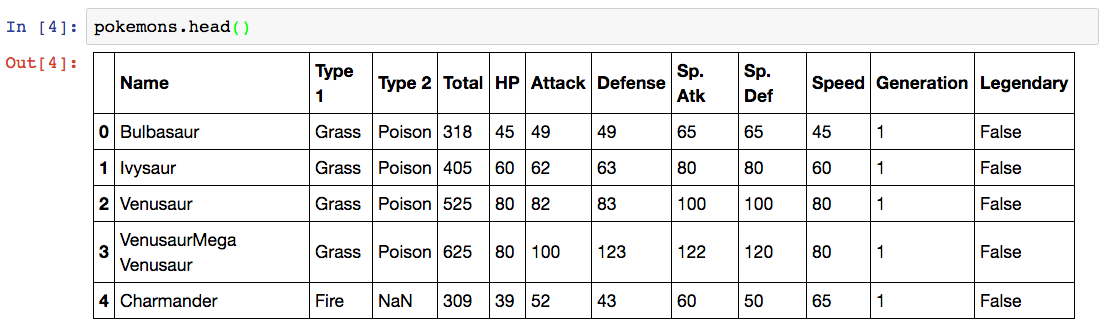
\includegraphics[width=\textwidth]{images/pokemons}
\end{frame}

\section{Какие признаки есть в датасете?}

\begin{frame}
	${f: X \rightarrow D_f}$
	\begin{enumerate} [-]
	  \item Бинарные (${D_f = \left\{ 0, 1 \right\} }$)
	  \item Номинальные (${D_f}$ -- конечное множество)
	  \item Порядковые (${D_f}$ -- конечное упорядоченное множество)
	  \item Количественные (${D_f = \mathbb{R} }$)
	\end{enumerate}
\end{frame}

\begin{frame}{Признаки}
	\begin{enumerate} [<+->]	
		\item[--] Бинарные (Legendary)
		\item[--] Номинальные (Type 1, Type 2)
		\item[--] Порядковые (Generation)
		\item[--] Количественные (Attack, Defense, ...)
	\end{enumerate}
\end{frame}

\begin{frame}{Легендарность}
\alert{Легендарный покемон} это чрезвычайно редкий и зачастую очень могущественных покемон, о нем слагаются мифы и легенды в мире покемонов.
\end{frame}

\begin{frame}{Легендарность}
	\begin{figure}
	    \centering
	    \subfloat{{
\includegraphics[width=2cm]{images/Bulbasaur} }}
	    \qquad
	    \subfloat{\frame{
\includegraphics[width=2cm]{images/Mewtwo} }}
    	    \qquad
    	    \subfloat{\frame{
\includegraphics[width=2cm]{images/Volcanion} }}
    	    \qquad
    	    \subfloat{{
\includegraphics[width=2cm]{images/Ekans} }}
    	    \qquad
    	    \subfloat{{
\includegraphics[width=2cm]{images/Nidorina} }}
	    \qquad 
    	    \subfloat{{
\includegraphics[width=2cm]{images/Rattata} }}
	    \qquad
    	    \subfloat{{
\includegraphics[width=2cm]{images/Sandshrew} }}
	    \qquad
    	    \subfloat{\frame{
\includegraphics[width=2cm]{images/Articuno} }}    	        	    
	\end{figure}
\end{frame}

\begin{frame}{Распределения}
  \centering
	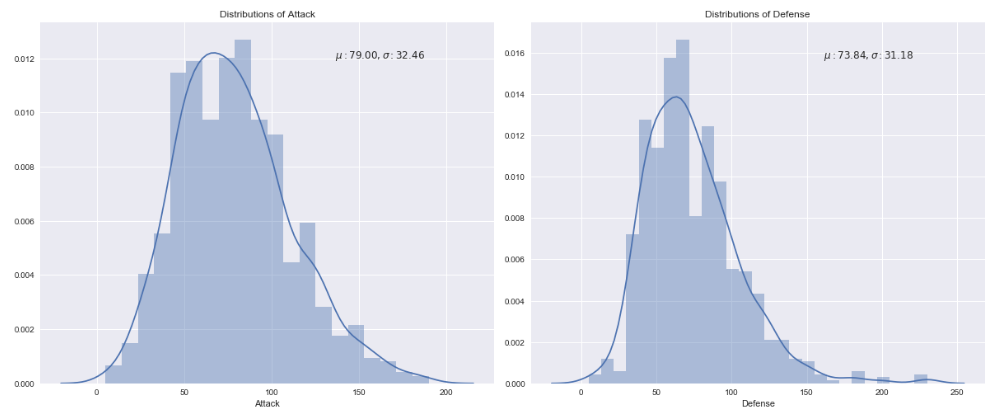
\includegraphics[width=\textwidth]{images/attack_defense}
	
	Number of Pokemons = 800
\end{frame}

{\foot{\href{https://github.com/ktisha/ML2017/tree/master/notebooks}{Репозиторий с материалами (https://github.com/ktisha/ML2017)}}
\begin{frame}{Типы покемонов}
  \begin{center}
	  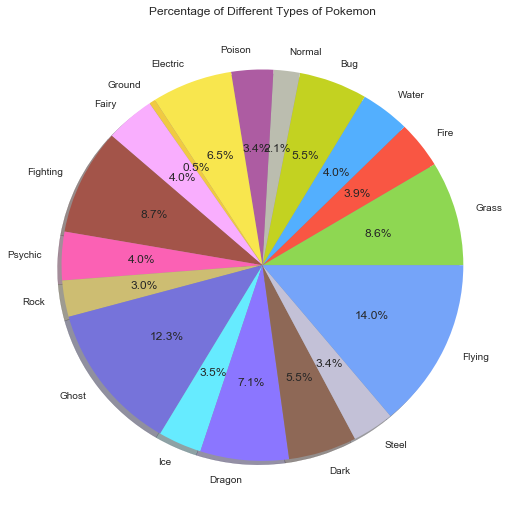
\includegraphics[width=\linewidth,height=0.8 \textheight,keepaspectratio]{images/pokemons_by_type}
  \end{center}
\end{frame}
}

\begin{frame}{Задача классификации}
	$X$ - множество объектов \\
	$Y$ - множество классов \\
	Обучающая выборка: ${X^l = (x_i, y_i)_{i=1}^l}$ \\ 
	\bigbreak
	\bigbreak
	\alert{Задача}: Построить алгоритм ${a \colon X \rightarrow Y}$, способный классифицировать произвольный объект ${x \in X}$.
\end{frame}

\begin{frame}{Задача классификации в нашем контексте}
	$X$ - покемоны \\
	$Y$ - легендарность \\
	Обучающая выборка: ${X^l = (x_i, y_i)_{i=1}^l}$ \\ 
	$l = 800$ покемонов в выборке\\
	\bigbreak
	\alert{Задача}: Построить алгоритм ${a \colon X \rightarrow Y}$, способный определить, является ли покемон легендарным.
\end{frame}

\section{Гипотеза компактности}

\begin{frame}{Гипотеза компактности}
  \centering
	Схожие объекты, как правило, лежат в одном классе.\\
	\bigbreak
	\uncover<2>{
    	Как определить \alert{схожесть} объектов?\\
   }
\end{frame}

\begin{frame}{Пример}
  \begin{center}
    	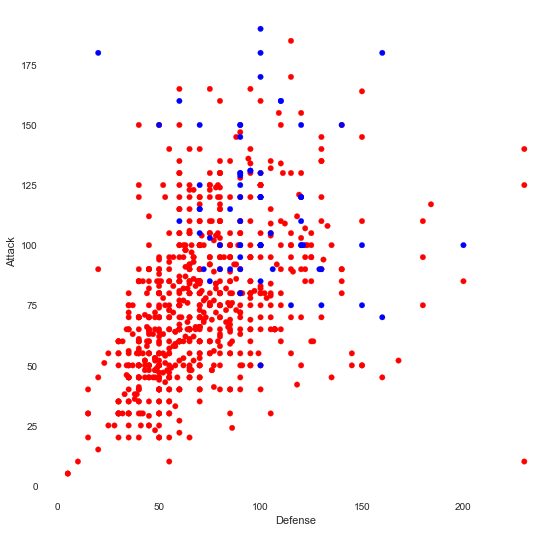
\includegraphics[width=\linewidth,height=0.8 \textheight,keepaspectratio]{images/attack_vs_defense}  
  \end{center}    
\end{frame}

\begin{frame}{Гипотеза компактности}
  \centering
	Схожие объекты, как правило, лежат в одном классе.\\
	\bigbreak
	\alert{Схожесть} $=$ Функция расстояния\\
	\bigbreak
	${\rho: X \times X \rightarrow [0, \infty) }$
\end{frame}

\section{Функции расстояния}

{\foot{Euclidean distance (metric)}
\begin{frame}{Евклидово расстояние}
	${\rho (u, v) = \sqrt{\sum\limits_{j=1}^n |u^j - v^j|^2}}$, \hspace{5mm} ${u, v \in X^{l}}$\\
	\bigbreak
	\bigbreak
	Признаковые описания объектов:\\
	${u = \left\{ u^1, u^2, ..., u^n \right\}}$ \\
	${v = \left\{v^1, v^2, ..., v^n \right\} }$ 
\end{frame}
}

{\foot{Манхэттенское расстояние, Taxicab distance}
\begin{frame}{Расстояние городских кварталов}
	${\rho (u, v) = \sum\limits_{j=1}^n |u^j - v^j|}$, \hspace{5mm} ${u, v \in X^{l}}$\\
	\bigbreak
	\bigbreak
	Признаковые описания объектов:\\
	${u = \left\{ u^1, u^2, ..., u^n \right\}}$ \\
	${v = \left\{v^1, v^2, ..., v^n \right\} }$ 
\end{frame}
}

{\foot{Minkowski distance}
\begin{frame}{Расстояние Минковского}
	Обобщение евклидова расстояния и расстояния городских кварталов
	\bigbreak
	${\rho (u, v) = (\sum\limits_{j=1}^n |u^j - v^j|^q)^{1/q}}$, \hspace{5mm} ${u, v \in X^{l}}$\\
	\bigbreak
	\bigbreak
	Признаковые описания объектов:\\
	${u = \left\{ u^1, u^2, ..., u^n \right\}}$ \\
	${v = \left\{v^1, v^2, ..., v^n \right\} }$ 
\end{frame}
}

{\foot{Редакционное расстояние, дистанция редактирования, Edit distance }
\begin{frame}{Расстояние Левенштейна}
	Минимальное количество операций вставки одного символа, удаления одного символа и замены одного символа на другой, необходимых для превращения одной строки в другую.
\end{frame}
}

\begin{frame}{Расстояние Левенштейна}
	\begin{center}
	  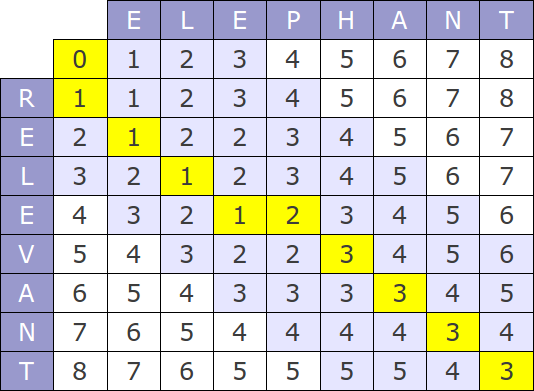
\includegraphics[width=\textwidth]{images/levenshtein}
	\end{center}
\end{frame}

\section{Метрический классификатор}

\begin{frame}{Обобщенный метрический классификатор}
	$u \in X$ - произвольный объект, который собираемся классифицировать.\\
	\bigbreak
	\pause
	Отсортируем объекты из $X^l$ относительно $u$:
	${\rho(u, x_1) \leq \rho(u, x_2) \leq \dots \leq \rho(u, x_l)}$\\
	\bigbreak
	${x_i}$ -- $i$-й сосед объекта $u$\\
	${y_i}$ -- класс $i$-го соседа $u$
\end{frame}

\begin{frame}{Обобщенный метрический классификатор}
	${\rho(u, x_1) \leq \rho(u, x_2) \leq \dots \leq \rho(u, x_l)}$\\
	\bigbreak
	${x_i}$ -- $i$-й сосед объекта $u$\\
	${y_i}$ -- класс $i$-го соседа $u$
  \bigbreak
  \uncover<2,3>{
    \alert{Идея 1}: Посмотрим на ближайшие объекты и отнесем $u$ к доминирующему классу. 
    }
  \uncover<3>{
  \bigbreak
  \alert{Идея 2}: Более близкие объекты важнее для классификации.
  }
\end{frame}

\begin{frame}{Метрический алгоритм классификации}
	$${a(u, X^l) = \arg\max\limits_{y \in Y} \sum\limits_{y_i = y} w(i, u)}$$\\
	\bigbreak
	\bigbreak	
	$w(i, u)$ - вес $i$-го соседа $u$, неотрицателен\\
\end{frame}

\begin{frame}{Метод ближайшего соседа}
	\boxed{{a(u, X^l) = \arg\max\limits_{y \in Y} \sum\limits_{y_i = y} w(i, u)}}
	\bigbreak
	Объект относится к тому классу, к которому относится ближайший в выборке.\\
	\bigbreak
	${w(i, u) = [i=1]}$\\
\end{frame}

\begin{frame}{Метод ближайшего соседа}
	\boxed{{a(u, X^l) = \arg\max\limits_{y \in Y} \sum\limits_{y_i = y} w(i, u)}}
	\bigbreak
	${w(i, u) = [i=1]}$\\
	\bigbreak
	\begin{itemize} [<+- | alert@+>]
		\item[+] Простота
		\item[+] Интерпретируемость решения
	  \bigbreak
		\item[--	] Неустойчивость к шуму
		\item[--	] Отсутствие настраиваемых параметров
		\item[--	] Низкое качество классификации
		\item[--	] Необходимость хранить всю выборку целиком		
	\end{itemize}
\end{frame}

\begin{frame}{Пример}
  \begin{center}
    	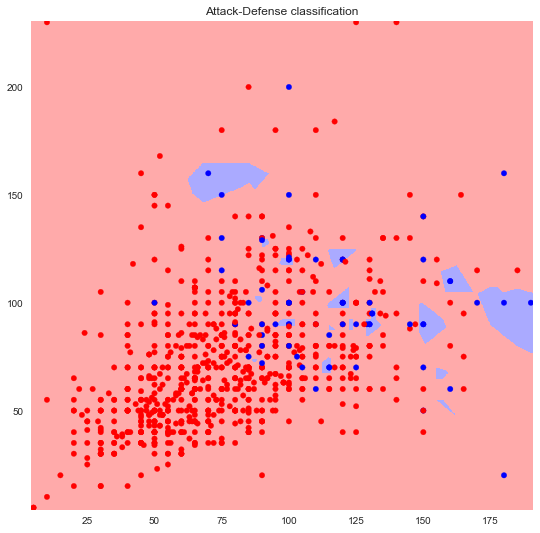
\includegraphics[width=\linewidth,height=0.8\textheight,keepaspectratio]{images/attack_vs_defense_fail}  
  \end{center}
\end{frame}

\begin{frame}{Метод k ближайших соседей}
  \boxed{{a(u, X^l) = \arg\max\limits_{y \in Y} \sum\limits_{y_i = y} w(i, u)}}
	\bigbreak
	${w(i, u) = [i \leq k]}$\\
	\bigbreak
	\begin{itemize} [<+- | alert@+>]
		\item[+] Менее чувствителен к шуму
		\item[+] Появляется настраиваемый параметр k
	  \bigbreak
	  \item[--] Неоднозначность при ${\sum\limits_{y_i = y} w(i, u) = \sum\limits_{y_i = s} w(i, u)}$ \hspace{5mm} $y \neq s$
	\end{itemize}
\end{frame}

\section{Подбор параметров}

\begin{frame}{Как выбрать $k$}
	Функционал скользящего контроля (leave-one-out):\\
	\bigbreak
	${LOO(k, X^l) = \sum\limits_{i=1}^l [a(x_i; X^l \backslash \left\{x_i\right\}, k) \neq y_i] \rightarrow \min\limits_k}$\\
\end{frame}

\begin{frame}{Вопрос}
  \centering
	Правда ли нужно выбрасывать один объект?
\end{frame}

\begin{frame}{Пример}
	\begin{center}
	  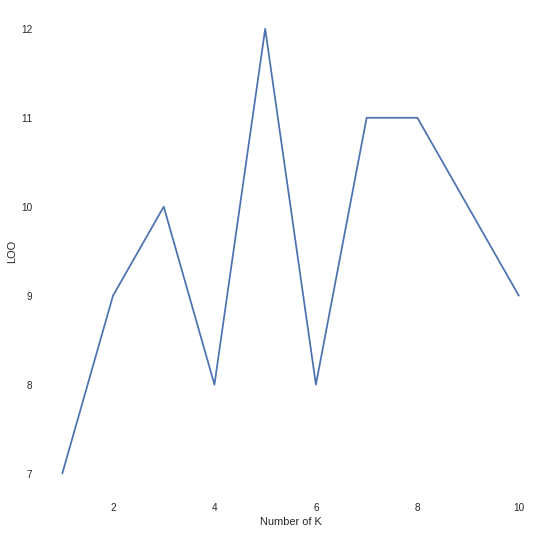
\includegraphics[width=\textwidth, height=0.8 \textheight, keepaspectratio]{images/loo}
	\end{center}
\end{frame}

\begin{frame}{Метод $k$ взвешенных соседей}
  \boxed{{a(u, X^l) = \arg\max\limits_{y \in Y} \sum\limits_{y_i = y} w(i, u)}}
  \bigbreak
	${w(i,u) = [i \leq k] * w_i}$, где $w_i$ это вес, зависящий только от номера соседа\\
	\bigbreak
	Возможные эвристики:\\	

	\begin{itemize} [<+->]
	\item ${w_i = \frac{k+1-i}{k}}$ -- линейное убывающие веса\\ % почему плохо?
	\item ${w_i = q^i}$ -- экспоненциально убывающие веса\\
	\end{itemize}
\end{frame}

\begin{frame}{Вопрос}
	\centering
	Как более обоснованно задать веса?\\
\end{frame}

{\foot{Kernel density estimation. Parzen–Rosenblatt window}
\begin{frame}{Ядерная оценка плотности}
	\textbf{Метод окна Парзена}\\
  $K(r)$ -- ядро, невозрастающее, положительное на ${[0, 1]}$\\
  \bigbreak
  \uncover<2,3>{
	Фиксированной ширины:\\
	${a(u, X^l, h, K) = \arg\max\limits_{y \in Y} \sum\limits_{y_i = y} K(\frac{\rho(u, x_i)}{h})}$  \hspace{5mm}  $h$ -- ширина окна\\
  \bigbreak
  }
  \uncover<3>{
    	Переменной ширины:\\
	  ${a(u, X^l, k, K) = \arg\max\limits_{y \in Y} \sum\limits_{y_i = y}  K(\frac{\rho(u, x_i)}{\rho(u, x_{k})})}$
	}
\end{frame}
}

\begin{frame}{Более наглядно}
    \centering
	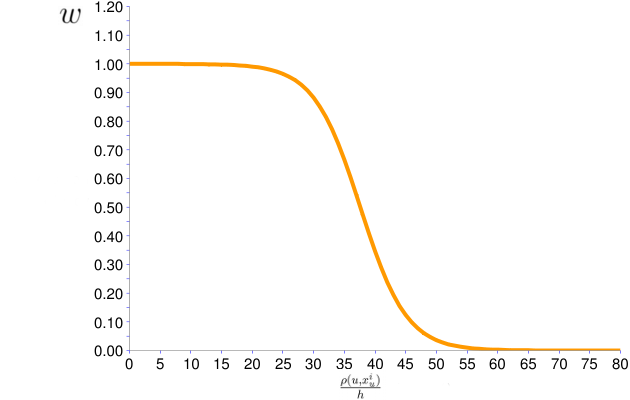
\includegraphics[width=\linewidth,height=\textheight,keepaspectratio]{images/parzen}
\end{frame}

\section{Выбор метрики}

\begin{frame}{Выбор метрики}
	\alert{Идея}: Максимизировать сумму расстояний между объектами разных классов
	при этом сохраняя сумму расстояний между объектами одного класса небольшой.\\
	\bigbreak
	\uncover<2,3>{
    $${\max \sum\limits_{x_i \in D, x_j \in F} \rho(x_i, x_j) } \qquad D \neq F$$	
	}
	\uncover<3>{
	\bigbreak
	$${\sum\limits_{x_i, x_j \in S} \rho^2(x_i, x_j) \leq 1 }$$
	}
\end{frame}

\begin{frame}{Проклятие размерности}
	\centering
	Если используемая метрика ${\rho(u, x_i)}$ основана на суммировании различий по всем признакам, а число признаков очень велико,
	то все точки выборки могут оказаться практически одинаково далеки друг от друга.\\
\end{frame}

\begin{frame}{Пример}
	\centering
	Набор признаков объекта генерируется подбрасыванием честной монетки $n$ раз. Соответственно
	каждый объект описывается вектором $[0, 1]^n$. При таких условиях все объекты будут равноудалены.
\end{frame}

\section{Предобработка}

\begin{frame}{Предобработка данных}
	\centering
	Что произойдет, если признаки представлены в разном масштабе?
\end{frame}

\begin{frame}{Предобработка данных}
	Все признаки должны быть представлены \alert{в одном масштабе}. \\
	В противном случае признак с наибольшими числовыми значениями будет доминировать в метрике.
\end{frame}

\begin{frame}{Жадное добавление признаков}
	\begin{enumerate} [<+->]
		\item ${\rho_j(u, x_i) = \vert u^j - x_i^j \vert}$ -- расстояние по j-му признаку\\
		          $LOO(j) \rightarrow \min$\\
		\item Добавляем признак и строим $\rho'$\\
							${\rho'(u, x_i) = \rho(u, x_i) + w_j\rho_j(u, x_i)}$\\
							$LOO(j, w_j) \rightarrow \min$\\
		\item Заменяем признак\\
            		${\rho'(u, x_i) = \rho(u, x_i) - w_k\rho_k(u, x_i) + w_j\rho_j(u, x_i)}$\\
		\item Добавляем признаки, пока LOO не увеличивается
	\end{enumerate}
\end{frame}

\begin{frame}{Сверхбольшие выборки}
	\begin{itemize} [<+- | alert@+>]
		\item[--] Проблема хранения
		\item[--] Проблема быстрого поиска ближайших соседей
	\end{itemize}
\end{frame}

\section{Отбор эталонов}

\begin{frame}\frametitle{Метрический алгоритм классификации}
	${a(u, X^l) = \arg\max\limits_{y \in Y} \underbrace{\sum\limits_{y_i = y} w(i, u)}_{\Gamma_y(u)} }$\\
	\bigbreak
	$w(i, u)$ - вес $i$-го соседа $u$, неотрицателен\\
	$\Gamma_y(u)$ - оценка близости объекта $u$ к классу ${y}$
\end{frame}

\begin{frame}{Отступ}
	${\Gamma_y(u) = \sum\limits_{y_i = y} w(i, u)}$ -- оценка близости объекта $u$ к классу ${y}$\\
	\bigbreak
	Отступ показывает степень \alert{типичности объекта}.\\
	\bigbreak
	\alert{Отступом} объекта ${x_i \in X^l}$ относительно классификатора $a$ называется величина:\\
	\bigbreak
	\centering	
  ${M(x_i) = \Gamma_{y_i}(x_i) - \max\limits_{y \in Y\backslash y_i} \Gamma_y(x_i)}$

\end{frame}

\begin{frame}{Типы объектов}
	\begin{enumerate} [<+->]
		\item Эталонные
		\item Надёжно классифицируемые (неинформативные)
		\item Пограничные	
		\item Ошибочные	
		\item Шумовые	
	\end{enumerate}
\end{frame}

{\foot{картинка с machinelearning.ru}
\begin{frame}{Типы объектов}
  \begin{center}
    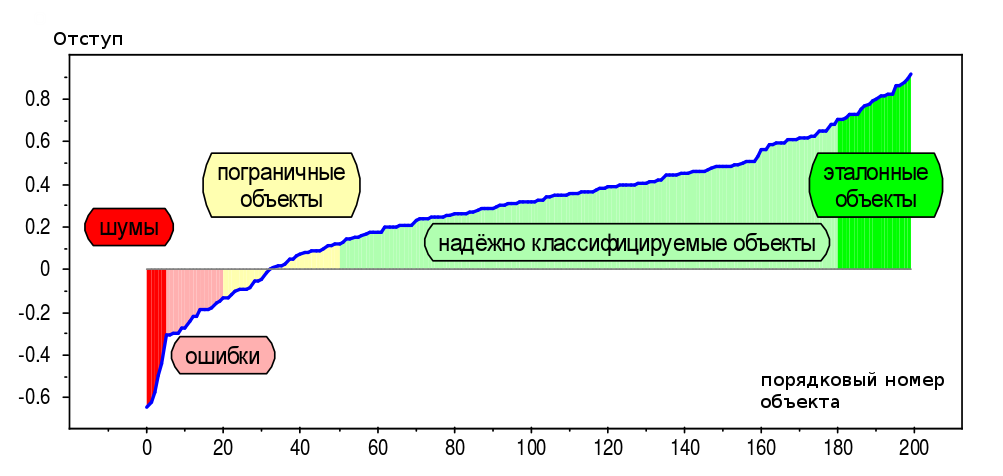
\includegraphics[width=\textwidth, keepaspectratio]{images/margin}
  \end{center}
\end{frame}
}

\begin{frame}{Отбор эталонных объектов}
	\alert{Задача}:\\
	Выбрать оптимальное подмножество эталонов $\Omega\subseteq X^l$\\ 
    \bigbreak
	Классификатор будет иметь вид:\\
	$${a(u, \Omega) = \arg\max\limits_{y \in Y} \sum\limits_{x_i \in \Omega} [y_i = y]w(i, u) }$$\\
\end{frame}

\begin{frame}{Алгоритм STOLP}
	\begin{enumerate}
		\item Исключить выбросы и пограничные объекты
		\item Найти по одному эталону в каждом классе
		\item Добавлять эталоны, пока есть отрицательные отступы	
	\end{enumerate}
\end{frame}

\begin{frame}{Алгоритм STOLP}
	\begin{itemize} [<+- | alert@+>]
	\item[+] Сокращается число хранимых объектов
	\item[+] Сокращается время классификации
	\item[+] Объекты разделяются по величине отступа
	\bigbreak
	\item[--] Выбор параметра для определения выбросов
	\item[--] Не высокая эффективность
	\end{itemize}
\end{frame}

\begin{frame}[standout]
  Вопросы?
\end{frame}

\appendix

\section{Быстрый поиск ближайших соседей}

\begin{frame}{Быстрый поиск ближайших соседей}
	\begin{enumerate} [--]
		\item граф ближайших соседей
		\item k-d дерево
		\item хеширование (LSH)
	\end{enumerate}
\end{frame}

\begin{frame}\frametitle{k-d дерево}
	\alert{Идея}: разложим множество по поторому будем искать в бинарное дерево с простыми условиями и конкретными точками в узлах.
	\bigbreak
	\uncover<2,3> {
	\begin{enumerate}
		\item По циклу, или рандомно выбираем ось.
		\item Ищем медиану (точку, разбивающую множество на как можно более равные части).
		\item Повторяем 1-2 для каждого из получившихся подмножеств 
	\end{enumerate}
	}
	\uncover<3>{
	Сложность построения: $O(n\log n)$\\
	Сложность поиска: в лучшем случае $O(\log n)$, в худшем -- $O(n)$
	}
\end{frame}

\begin{frame}\frametitle{2-d дерево}
	\begin{center}
    	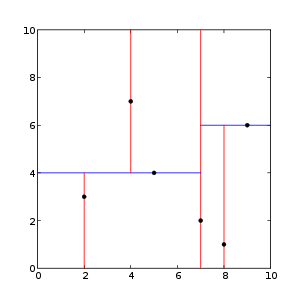
\includegraphics[height=190pt]{images/Kdtree_2d}  	
	\end{center}
\end{frame}

\begin{frame}\frametitle{k-d дерево. Особенности}
	\begin{itemize} [<+- | alert@ +>]
	\item[+] Один из наиболее простых методов
	\item[--] Работает только при малом количестве параметров
	\item[--] Затратный алгоритм перестроения
	\end{itemize}
\end{frame}

\begin{frame}\frametitle{Locality Sensitive Hash}
  \alert{Задача}: Найти похожие документы в интернете\\
\end{frame}

\begin{frame}\frametitle{Locality Sensitive Hash}
	\alert{Проблема}: Сколько сравнений нам понадобится  для того, чтобы найти похожие среди $N$ документов?\\
	\bigbreak
	\uncover<2>{
	$C = \frac{N(N-1)}{2}$\\
	\bigbreak
	$N = 10^6 \Rightarrow C = 5*10^{11}$
	}
\end{frame}

\begin{frame}\frametitle{Locality Sensitive Hash}
	\alert{Идея}: Давайте от каждого документа (строки из нулей и единиц) возьмем хэш $h$:\\
	\begin{enumerate} [<+->]
	\item Если документы $C_1$ и $C_2$ похожи, то с большой вероятностью $h(C1) == h(C2)$\\
	\item Иначе -- с большой вероятностью $h(C1) \neq h(C2)$
	\end{enumerate}
\end{frame}

\begin{frame}\frametitle{Locality Sensitive Hash}
	\alert{Идея}: \\
	\begin{enumerate}
	\item Разбить документ на n-граммы
	\item Взять от каждого n-грамма хэш
	\item Получим представление документа в виде строки из нулей и единиц. Длина такого вектора = количество всевозможных n-грамм.
	\item Посчитаем документы похожими, если у них много совпадающих n-грамм
	\end{enumerate}
\end{frame}

\begin{frame}\frametitle{Locality Sensitive Hash}
	\begin{figure}[htbp]
	\centering
	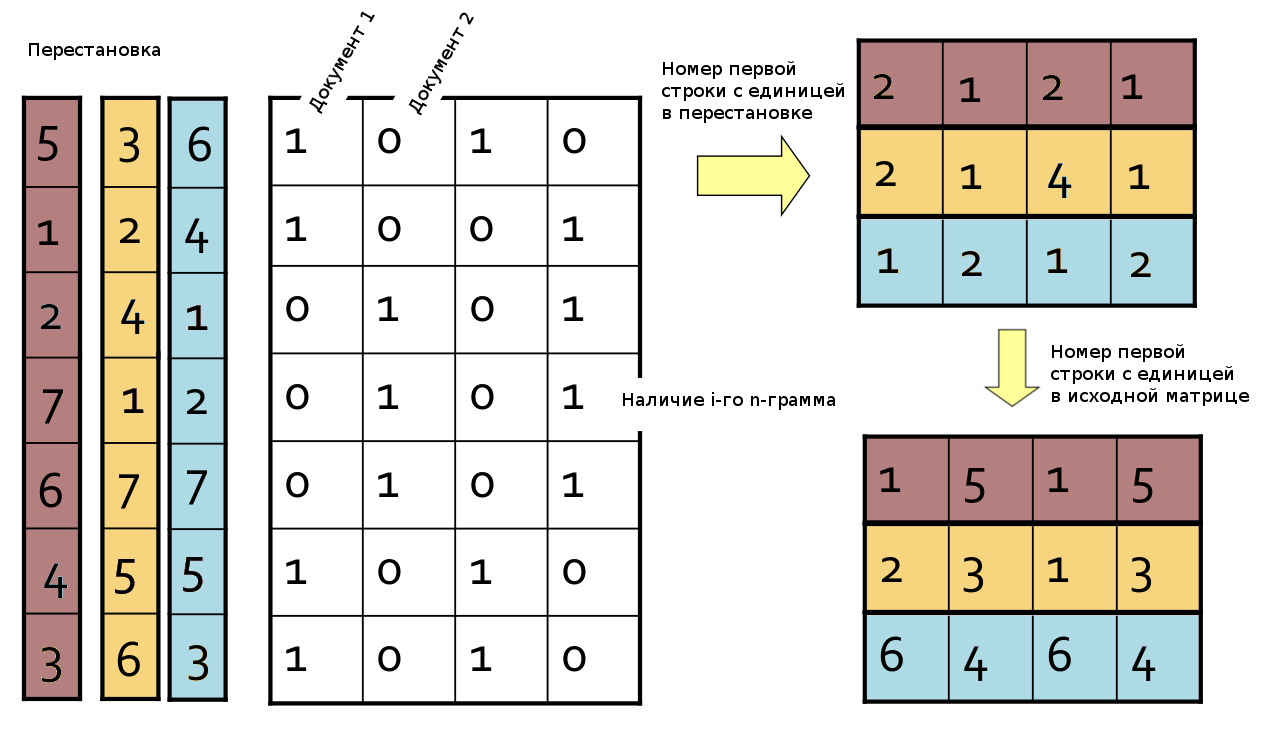
\includegraphics[height=190pt]{images/min-hash1}  
	\end{figure}
\end{frame}

\begin{frame}\frametitle{Что происходит сейчас в области knn}
  ICML'16: \href{http://jmlr.org/proceedings/papers/v48/lic16.pdf}{Fast $k$-Nearest Neighbour Search via Dynamic Continuous Indexing}\\
  \bigbreak
  NIPS'16: \href{http://papers.nips.cc/paper/6373-k-nearest-neighbors-from-global-to-local.pdf}{$k^\ast$-Nearest Neighbors: From Global to Local}\\
  \bigbreak
  NIPS'16: \href{http://papers.nips.cc/paper/6123-finite-sample-analysis-of-fixed-k-nearest-neighbor-density-functional-estimators.pdf}{Finite-Sample Analysis of Fixed-$k$ Nearest Neighbor Density Functional Estimators}\\
\end{frame}

\begin{frame}\frametitle{На следующей лекции}
	\begin{enumerate} [--]
		\item Кластеризация.  K-means.
		\item Цели кластеризации.
		\item Типы кластерных структур.
		\item Функционал качества кластеризации
		\item К-средних
		\item Иерархическая кластеризация.
	\end{enumerate}
\end{frame}

\end{document}

              
